\begin{marginfigure} % MARGIN FIGURE
\begin{center}
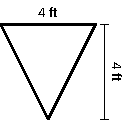
\includegraphics[scale=1.5]{figures/figfluid2a}
\end{center}
\caption{A thin plate in the shape of an isosceles triangle in Example \ref{eg:6.5.8}.} \label{F:6.5.triangle1}
\end{marginfigure}

\begin{example} \label{eg:6.5.8} % EXAMPLE
Consider a thin plate in the shape of an isosceles triangle as shown in Figure \ref{F:6.5.triangle1} submerged in water with a weight--density of 62.4 lb/ft$^3$. If the bottom of the plate is 10 ft below the surface of the water, what is the total fluid force exerted on this plate?


\solution
We approach this problem in two different ways. First we will let $y=0$ represent the surface of the water, then we will consider an alternate convention.
	\begin{enumerate}
	\item		We let $y=0$ represent the surface of the water; therefore the bottom of the plate is at $y=-10$. We center the triangle on the $y$-axis as shown in Figure \ref{F:6.5.triangle2}. The depth of the plate at $y$ is $-y$ as indicated by the Key Idea. We now consider the length of the plate at $y$.
		
	We need to find equations of the left and right edges of the plate. The right hand side is a line that connects the points $(0,-10)$ and $(2,-6)$: that line has equation $x=1/2(y+10)$. (Find the equation in the familiar $y=mx+b$ format and solve for $x$.) Likewise, the left hand side is described by the line $x=-1/2(y+10)$. The total length is the distance between these two lines: $\ell(y)=1/2(y+10) - (-1/2(y+10)) = y+10.$
	
The total fluid force is then:
\begin{align*}
F 	&=	\int_{-10}^{-6} 62.4(-y)(y+10)\ dy \\
		&=	62.4\cdot \frac{176}{3} \approx	3660.8\text{ lb}.
\end{align*}

\item		Sometimes it seems easier to orient the thin plate nearer the origin. For instance, consider the convention that the bottom of the triangular plate is at $(0,0)$, as shown in Figure \ref{F:6.5.triangle3}. The equations of the left and right hand sides are easy to find. They are $y=2x$ and $y=-2x$, respectively, which we rewrite as $x= 1/2y$ and $x=-1/2y$. Thus the length function is $\ell(y) = 1/2y-(-1/2y) = y$. 

As the surface of the water is 10 ft above the base of the plate, we have that the surface of the water is at $y=10$. Thus the depth function is the distance between $y=10$ and $y$; $d(y) = 10-y$. We compute the total fluid force as:
\begin{align*}
F	&=\int_0^4 62.4(10-y)(y)\ dy \\
	&\approx 3660.8\text{ lb}.
\end{align*}
\end{enumerate}
The correct answer is, of course, independent of the placement of the plate in the coordinate plane as long as we are consistent.
\end{example}

\begin{marginfigure}[-22cm] % MARGIN FIGURE
\begin{center}
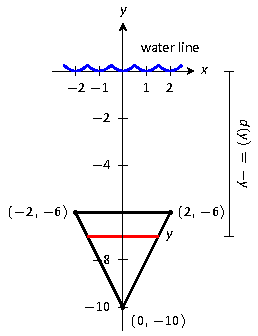
\includegraphics{figures/figfluid2b}
\end{center}
\caption{Sketching the triangular plate in Example \ref{eg:6.5.8} with the convention that the water level is at $y=0$.} \label{F:6.5.triangle2}
\end{marginfigure}

\begin{marginfigure}[-8cm] % MARGIN FIGURE
\begin{center}
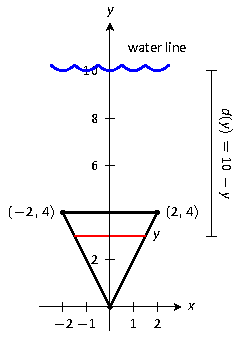
\includegraphics{figures/figfluid2c}
\end{center}
\caption{Sketching the triangular plate in Example \ref{eg:6.5.8} with the convention that the base of the triangle is at $(0,0)$.} \label{F:6.5.triangle3}
\end{marginfigure}